\section{Lexical and distributional semantics}
\begin{itemize}
	\item \textbf{Compositional semantics}: meaning of phrase/sentence
	\item \textbf{Lexical semantics}: meaning of individual words
\end{itemize}
\subsection{Approaches for lexical meaning}
\begin{itemize}
	\item How to represent a meaning of a word. Problem: no representation can fully capture language yet!
\end{itemize}
\subsubsection{Formal semantics}
\begin{itemize}
	\item Based on set theory, describing the features of a word
	\item Meaning postulates: $\forall x \left[\text{bachelor}'(x)\to\text{man}'(x)\wedge\text{unmarried}'(x)\right]$
	\begin{itemize}
		\item If a word is in the set \textit{bachelor}, then it also is in \textit{man} and \textit{unmarried}
	\end{itemize}
	\item Problems:
	\begin{itemize}
		\item Limited, especially for special cases (i.e. what is the Pope?)
		\item Very expensive for large corpus
		\item For some words, it is almost impossible to find a good formalization
	\end{itemize}
	\item Alternative: \textbf{Prototype theory}
	\begin{itemize}
		\item Notion of graded semantic categories with no clear boundaries
		\item No requirement that a feature must be shared by all members
		\item Certain members are more central or prototypical $\Rightarrow$ \textbf{Protoypes}
		\item New members are added based on similarity to prototypes
		\item Features and category memberships are graded
	\end{itemize}
\end{itemize}
\subsubsection{Semantic relations}
\begin{itemize}
	\item \textbf{Hyponymy}: IS-A relation, forms a taxonomy (\textit{Example}: dog is a hyponym of animal)
	\begin{itemize}
		\item Easier to construct for certain nouns, but especially hard for adjectives
	\end{itemize}
	\item \textbf{Meronomy}: PART-OF relation (\textit{Example}: arm is a meronym of body)
	\item \textbf{Synonymy}: Words can be exchanged without changing the meaning of a sentence/phrase
	\item \textbf{Antonymy}: Opposite meanings (\textit{Example}: big vs. little)
\end{itemize}
\subsubsection{WordNet}
\begin{itemize}
	\item Large-scale corpus for English resource
	\item Handconstructed
	\item Organized in synsets: sets of synonyms
	\item Synsets are connected by semantic relations
	\item Similarity of words is the similarity of synsets
\end{itemize}

\subsection{Polysemy and word sense disambiguation}
\begin{itemize}
	\item A word can mean different things based on the sentence/context it is used in
	\item Meaning of words is not fixed, but dynamically adapted by the context
	\item \textbf{Regular polysemy}: mechanisms to apply on words to fit into context
	\begin{itemize}
		\item \textit{Zero-derivation}: verb $\leftrightarrow$ noun without changing word. Example: ``\textit{tango}''
		\item \textit{Metaphorical}: using words from a different domain to express similar meaning. Example: ``\textit{swallow information}''
		\item \textit{Metonymy}: use an entity to actually refer to other aspects of it. 
		Example: ``\textit{drinking his glass}''
	\end{itemize}
	\item \textbf{Word sense disambiguation}: derive meaning of word in context
	\begin{itemize}
		\item \textit{Supervised} (most common) $\to$ predefined list of senses (i.e. WordNet), and train model on \textit{large} corpus. Problem: we have to learn a new classifier for every word!
		\item \textit{Semi-supervised} $\to$ annotate small dataset, bootstrap from there. Might be helpful as some instances have no single/discrete meaning.
		\item \textit{Unsupervised} $\to$ induce sense by clustering of word occurences. Usually, the result is either too fine-grained or coarse-grained for most word (only work great for frequent words)
	\end{itemize}
\end{itemize}
\subsubsection{Semi-Supervised WSD: Yarowsky algorithm}
\begin{itemize}
	\item Using bootstrapping which needs only a very small hand-labeled training set
	\item Still, learns a classifier for every word $\Rightarrow$ no generalization!
	\item Also, define features (see notion of context) for every word to determine its meaning
	\item \textbf{Algorithm iteration}: 
	\begin{enumerate}[start=0]
		\item Given a small initial seed set $\Lambda_0$ of labeled instances of each sense, and a much larger unlabeled corpus $V_0$
		\item Train classifier on $\Lambda_0$
		\item Use trained classifier to label $V_0$
		\item Select the examples in $V_0$ that the classifier is most confident on
		\begin{enumerate}
			\item Reliability of a prediction defined as $\log\left(\frac{p(a|w)}{p(b|w)}\right)$ for word w and possible senses $a$ and $b$
			\item Rank reliabilities of all predictions and choose $n$ best
		\end{enumerate}
		\item Remove chosen examples from $V_0\Rightarrow V_1$, and add them to the training set $\Rightarrow\Lambda_1$
		\item Repeat step 2) to 4) until:
		\begin{enumerate}
			\item Either $V_i$ is empty
			\item Or the error rate on the training/validation is sufficient low
		\end{enumerate}
	\end{enumerate}
	\item Reported accuracy of 95\%, but on easy homonymous examples
	\item \textbf{One sense per discourse}
	\begin{itemize}
		\item Original algorithm uses \textit{one sense per discourse} as second heuristic
		\item If a word appears twice or more often in the same text, they are probably of the same meaning\\
		$\Rightarrow$ Annotate these as well and use them as additional training examples
	\end{itemize}
\end{itemize}
\subsection{Distributional semantics}
\begin{itemize}
	\item Probabilistic models for semantics
	\item Distributional hypothesis about word meaning: the meaning of a word is determined by its context $\Rightarrow$ similar meanings have similar contexts
	\item Thus, distributions are a good conceptual representation if you believe that ‘the meaning of a word is given by its usage’ $\Rightarrow$ Corpus-dependent like different culture, domains, ...
	\item Distributions can encode lexical- and world knowledge, but mostly only partial lexical semantics 
	\item Techniques: Count-based models and prediction models
\end{itemize}
\subsubsection{Count-based models}
\begin{itemize}
	\item Vector spaced models in the semantic space, where every dimension corresponds to a possible context $\Rightarrow$ features
	\item Distribution can be seen as point in space
	\item As a result, we get a feature matrix:
	$$\begin{array}{c|cccc}
	& \text{feature}_1 & \text{feature}_2 & \dots & \text{feature}_n\\
	\hline
	\text{word}_1  & f_{1,1} & f_{2,1} & \dots & f_{n,1}\\
	\text{word}_2  & f_{1,2} & f_{2,2} & \dots & f_{n,2}\\
	\vdots  & \vdots & \vdots & \ddots & \vdots\\
	\text{word}_m  & f_{1,m} & f_{2,m} & \dots & f_{n,m}\\
	\end{array}$$
	\item Possible design choices in count-based models:
\end{itemize}
\begin{enumerate}
	\item \textbf{Notion of context}: how to define the context of a word
	\begin{enumerate}
		\item \textit{Word windows}: n words on either side of the lexical item, and count occurrences of words
		\item \textit{Filtered word windows}: n words, but remove irrelevant words based on POS-tag or stop-list (don't need to extend window)
		\item \textit{Lexeme windowing}: word windows (filtered or unfiltered), but with using stemming (mostly lead to more robust models)
		\item \textit{(Syntactic) dependencies}: context with dependency structure it belongs to (directed link between heads and dependents). Can be used with different extends\\
		Example: ``The prime minister acknowledged the question'' \\
		- [prime\_a 1, acknowledge\_v 1] (a for adjectives, v for verbs)\\
		- [prime\_a\_mod 1, acknowledge\_v\_subj 1] (mod for modifiers, subj for verb in relation to subject)\\
		$\Rightarrow$ Problem: complex context lead to sparse vectors
	\end{enumerate}
	$\Rightarrow$ Working best: small window sizes or short dependencies
	\item \textbf{Context weighting}: how to set the weights in the vector
	\begin{enumerate}
		\item \textit{Binary model}: if $c$ co-occurs with word $w$, value of entry is 1, else 0
		\item \textit{Basic frequency model}: number of times $c$ co-occurs (probably normalized)
		\item \textit{Characteristic model}: weights express how characteristic a given context is for a word $w$\\
		\item \textit{Pointwise Mutual Information (PMI)}: example of characteristic model. Comparing probability of both words occur together compared to occurring alone.\\
		$$PMI(w,c)=\log \frac{P(w,c)}{P(w)P(c)} = \log \frac{P(c|w)}{P(c)} \text{\hspace{5mm} where \hspace{5mm}}P(c) = \frac{f(c)}{\sum_k f(c_k)}, P(c|w) = \frac{f(w,c)}{f(w)}$$
		$$\Rightarrow PMI(w,c) = \log \frac{f(w,c)\sum_k f(c_k)}{f(w)f(c)}$$
		$PPMI\to$ only use positive values, $PPMI(w,c) =\max\left(PMI(w,c),0\right)$
	\end{enumerate}
	\item \textbf{Semantic space}: what are possible contexts
	\begin{enumerate}
		\item \textit{Entire vocabulary}: every word represents a possible context.\\
		+ All info included (also the rare one) - Inefficient (large space \& sparse), noisy
		\item \textit{Top n words with highest frequency}: \\
		+ More efficient, noise is filtered out - May miss out infrequent contexts
		\item \textit{Singular Value Decomposition}: dimension reduction by exploiting redundancies\\
		+ Very efficient, good generalization - Not interpretable (or very hard)
		\item \textit{Non-negative matrix factorization}: Similar to SVB, but performs factorization differently
	\end{enumerate}
\end{enumerate}
\subsubsection{Prediction-based models}
\begin{itemize}
	\item Train a model to predict plausible contexts for a word
	\item Learn word representations in the training process
	\item \textbf{Short dense} embeddings with \textbf{latent} dimensions 
	\begin{itemize}
		\item Easier to use as features with machine learning
		\item Better generalization than simple counting $\Rightarrow$ capturing more complex relations like synonym
	\end{itemize}
	\item One example for prediction-based models is skip-gram, also known as word2vec (see later section)
\end{itemize}
\subsubsection{Similarity}
\begin{itemize}
	\item Definition of similarity very broad. Can include synonym, antonyms, hyponyms, ...
	\item Measuring similarity with \textbf{Cosine} between vectors $v$ and $u$:
	$$\cos\left(\theta\right) = \frac{\sum_k v_k \cdot u_k}{\sqrt{\sum_k v_k^2} \cdot \sqrt{\sum_k u_k^2}}$$
	\item Cosine measure calculates the angle between $v$ and $u$, and is length-independent (normalization). Important as frequent words can have longer vectors
	\item Other measures include Jaccard, Euclidean distance (vectors need to be normalized!), ...
	\item However, true-synonyms do not always get higher similarity scores than near-synonyms, and also to antonyms
	\item Identifying antonyms by extra heuristics like checking words with high similarity that frequently appear together (\textit{example}: ``we serve hot and cold drinks'')
	
\end{itemize}
\subsubsection{Distributional word clustering}
\begin{itemize}
	\item Cluster words based on the contexts they occur
	\item Predefine number of clusters and corpus (for instance 2000 nouns in 200 clusters)
	\item \textbf{Features} can represent different kinds of contexts
	\begin{itemize}
		\item Windows based context, parsed or unparsed, syntactic dependencies
		\item Define notion of context, context weighting, and semantic space 
		\item Feature representation can significantly influence performance
	\end{itemize}
	\item Clustering algorithm: K-means
	\begin{itemize}
		\item Given dataset with $N$ points and task of $K$ clusters, minimize sum of squares of distance of each data point to its closest cluster mean $\bm{\mu}_i$:
		$$\arg\min_C \sum\limits_{i=1}^{K}\sum\limits_{\bm{x}\in C_i} ||\bm{x} - \bm{\mu}_{i}||^2$$
	\end{itemize}
	\item Small context sizes (small windows, syntactic dependencies) lead to clusters of synonyms (words that can be replaced)
	\item Large context sizes lead to \textbf{topical similarity} (words belonging to the same topic)
\end{itemize}

\subsubsection{Skip-gram}
\begin{itemize}
	\item Sometimes referred to as \textit{word2vec} because it is implemented in this package
	\item Given a word $w_t$, predict neighbouring words in a context windows of $2L$ words (for $L=2$: $w_{t-2}, w_{t-1}, w_{t+1}, w_{t+2}$) 
	\item In skip-gram, we learn two representations for every word $w_j \in V$:
	\begin{itemize}
		\item \textbf{word embedding} $v$ in word matrix $W$
		\item \textbf{context embedding} $c$ in context matrix $C$ (word in the role as context for other words)
	\end{itemize}
	\item To learn these embeddings, we take every word $w(t)$ in the corpus (index $j$ in vocabulary), and try to predict $w(t+1), ...$ where we denote this word with index $k$ in the vocabulary: 
	$$p\left(w_k | w_j\right)$$
	\item The idea in skip-gram is that we compute this probability by the similarity between the words $w_k$ and $w_j$ whereas we use the context matrix $C$ for $w_k$ and the word matrix $W$ for $w_j$ (see figure below)
	\begin{figure}[ht]
		\centering
		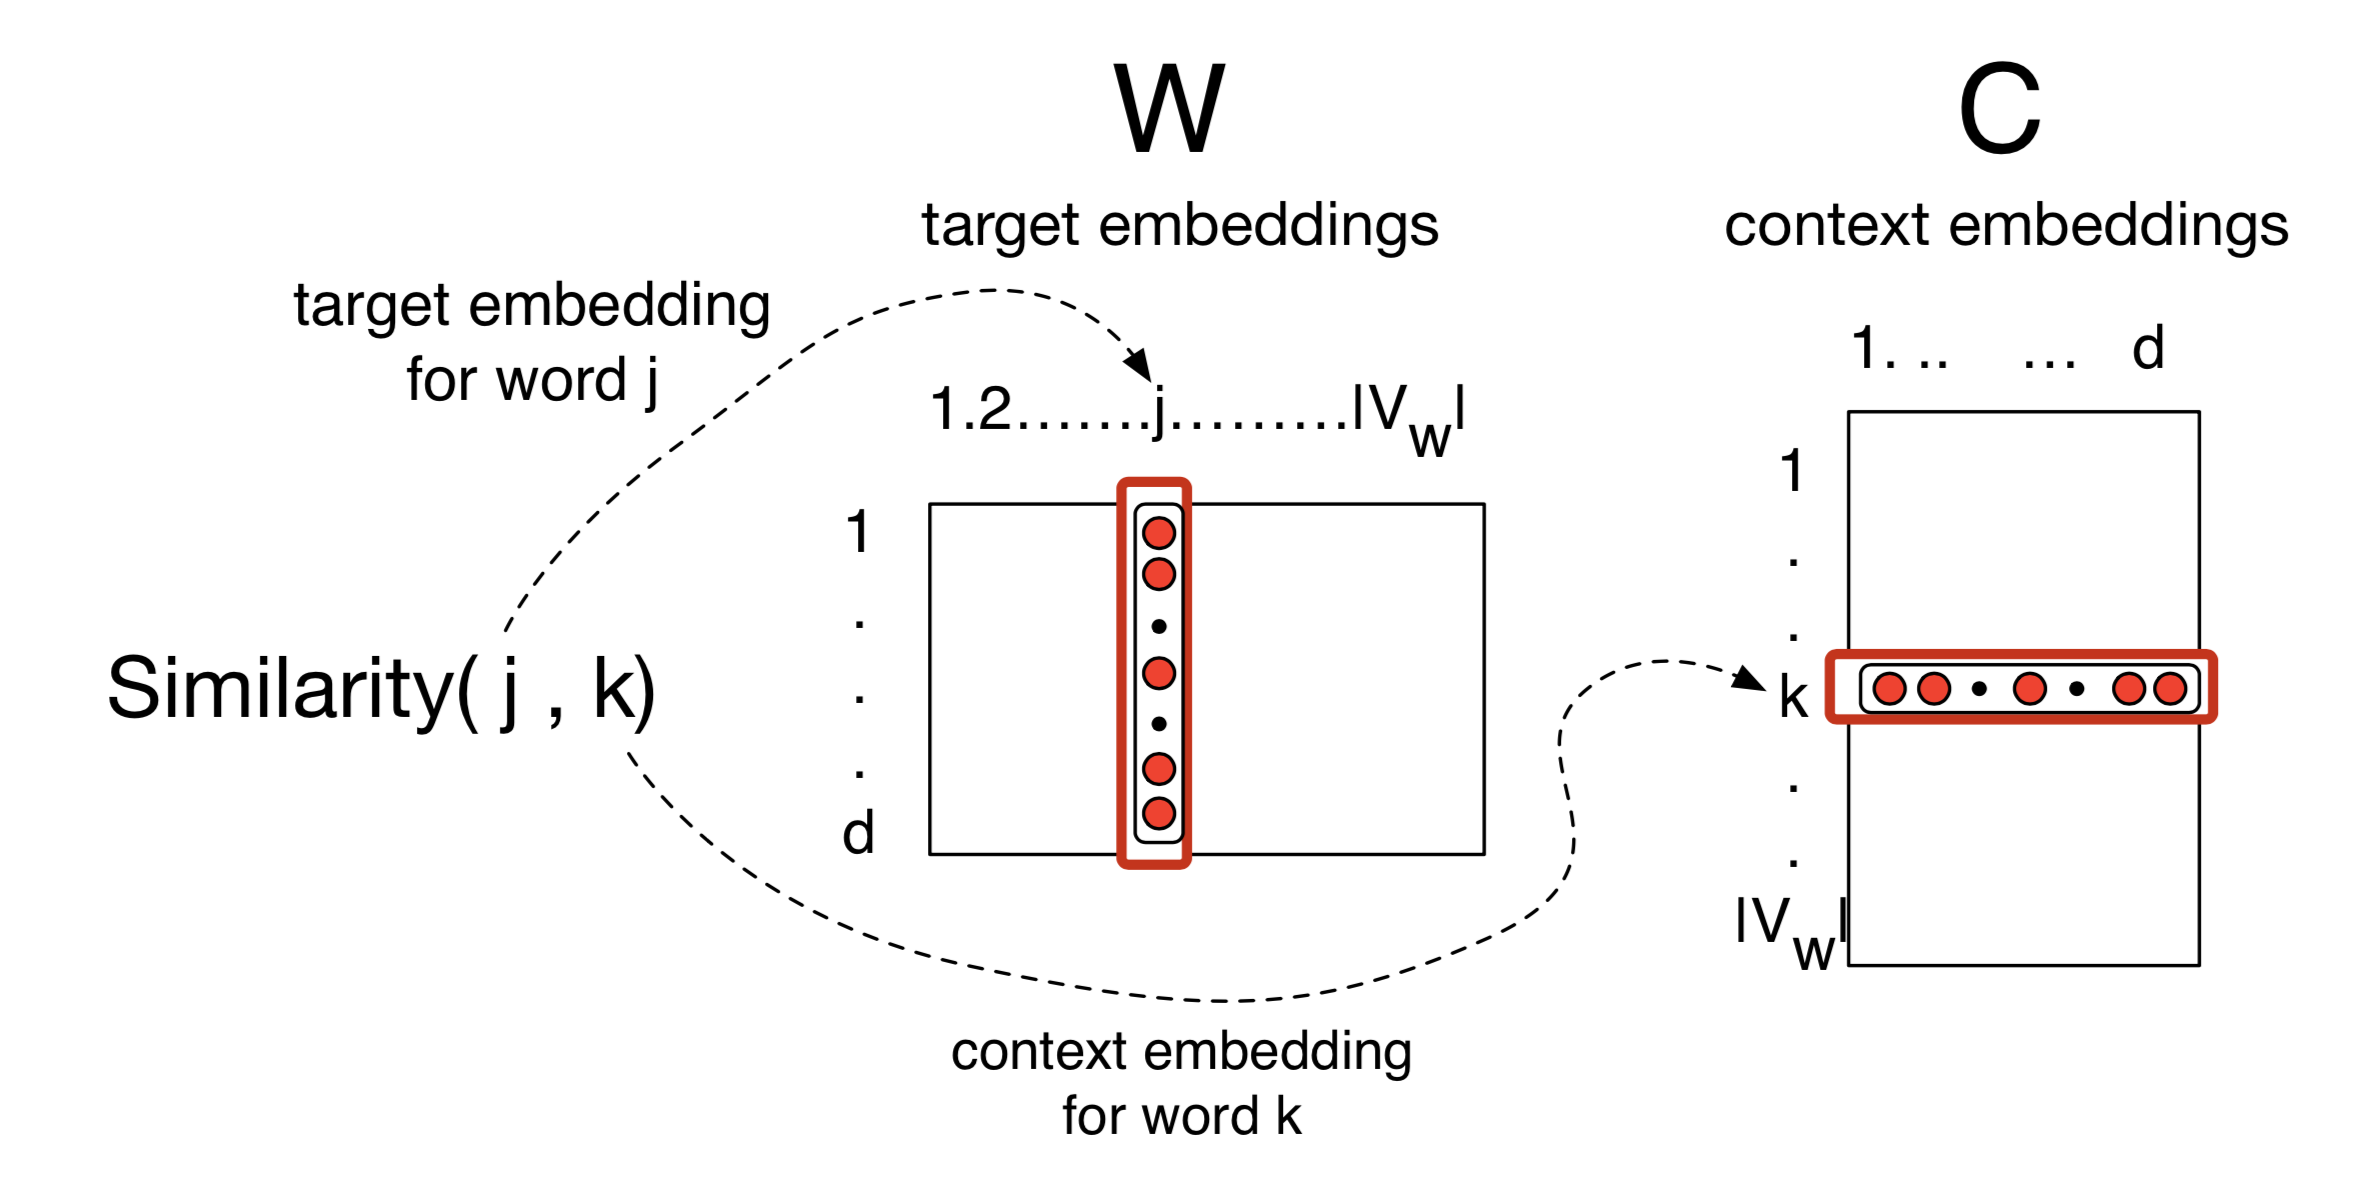
\includegraphics[width=0.5\textwidth]{figures/skip_gram_matrices.png}
		\caption{Skip gram overview}
		\label{fig:skip_gram_matrices}
	\end{figure}
	\item Similar to the cosine similarity, we use the dot product for calculating this:
	$$\text{Similarity}(c_k, v_j)\propto c_k\cdot v_j$$
	\item To normalize and get probability distribution over contexts, we use the softmax function:
	$$p\left(w_k|w_j\right)=\frac{\exp\left(c_k \cdot v_j\right)}{\sum_{i\in V} \exp\left(c_i \cdot v_j\right)}$$
	\item For the learning process, we start with randomly initialized vectors, and try to maximize the log-likelihood of the dataset (by performing SGD or similar):
	$$\arg\max \sum\limits_{\left(w_j, w_k\right)\in D} \log p\left(w_k|w_j\right) = \sum\limits_{\left(w_j, w_k\right)\in D}  \left(c_k \cdot v_j - \log \sum\limits_{c_i \in V} \exp\left(c_i \cdot v_j\right)\right)$$
	\item We can also represent skip-gram as a (neural) network:
	\begin{figure}[ht]
		\centering
		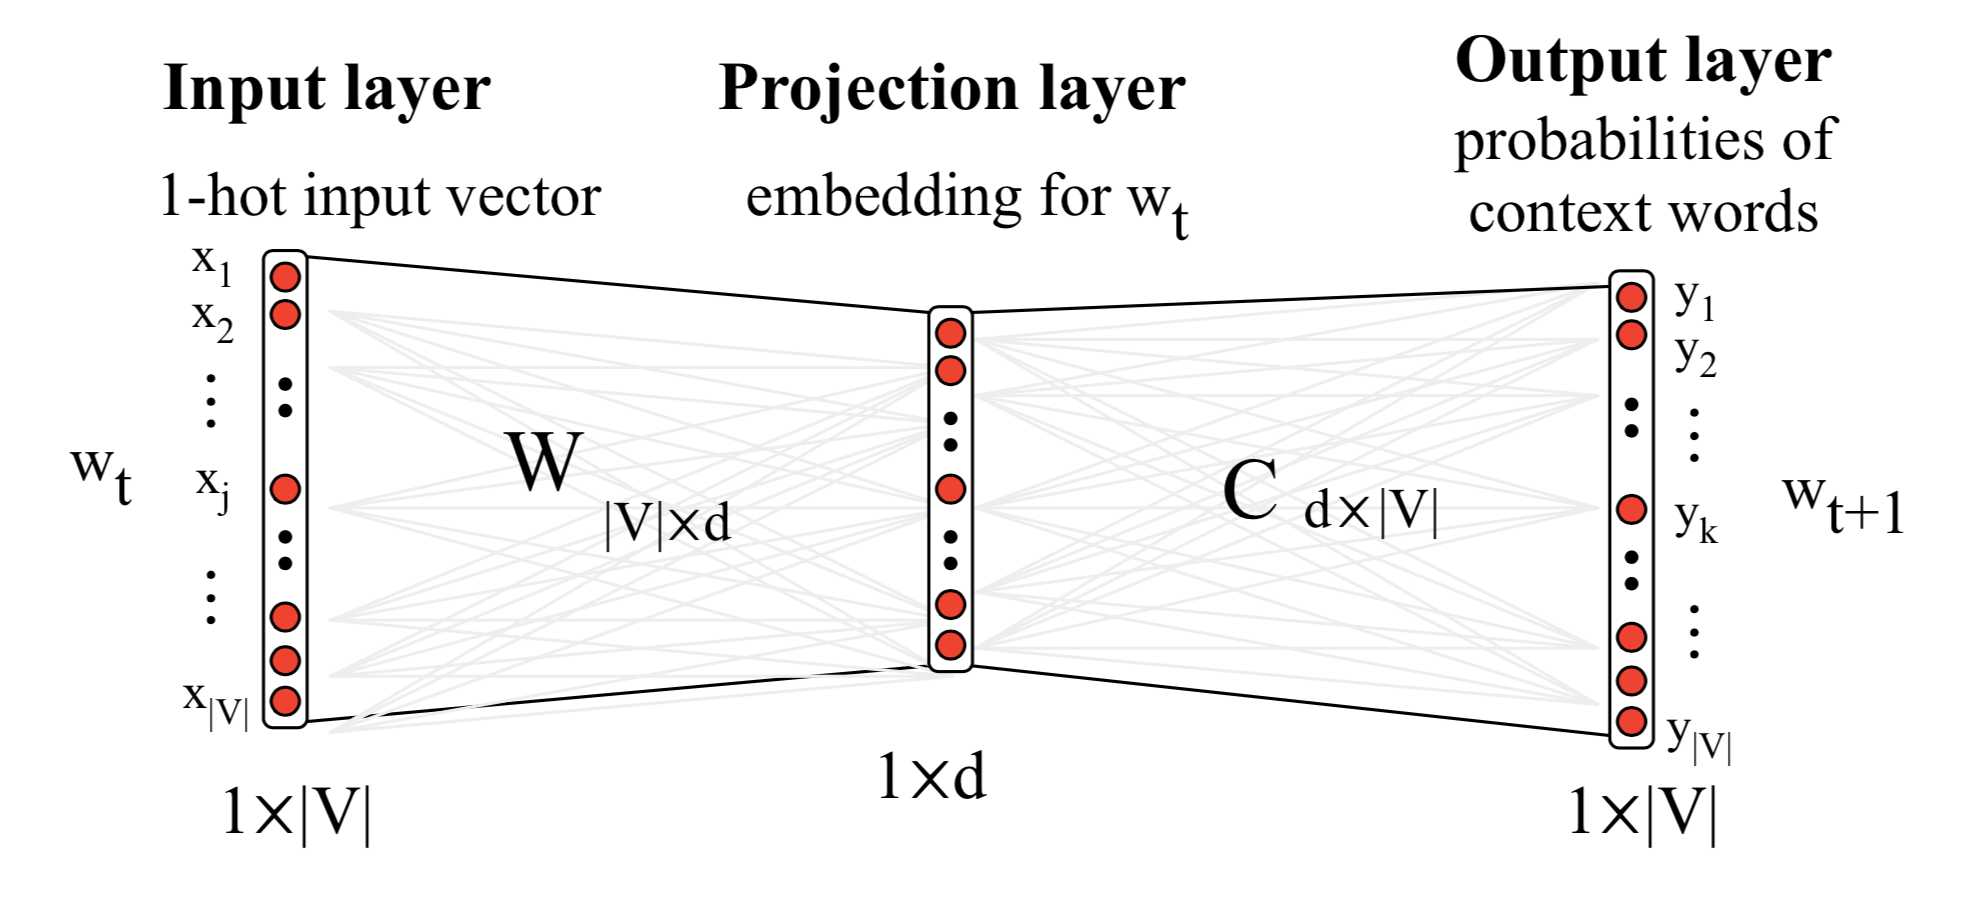
\includegraphics[width=0.5\textwidth]{figures/skip_gram_nn.png}
		\caption{Skip gram as neural network. The weights of the first layer represent the word embedding $W$, whereas the context embedding $C$ is in the second layer.}
		\label{fig:skip_gram_nn}
	\end{figure}
	\item However, the problem here is that for a large vocabulary size, the denominator of the softmax is very expensive to calculate $\Rightarrow$ \textbf{negative sampling}
	\begin{itemize}
		\item Approximate denominator by sampling $k$ random words from vocabulary (probability of sampling for a word is mostly connected to its unigram probability/frequency in the corpus like $\text{count}^{\alpha}(w)$ with for example $\alpha=0.75$)
		\item Dataset consists therefore out of words pair which are either positive or negative examples for context + word (note that we do not distinguish between the probability calculation of $w_{t-2}$ and $w_{t-1}$ for example)
		\item We convert the classification task into predicting whether a context pair is a positive or negative example from the corpus
		$$p\left(+|w_j, w_k\right) = \sigma(c_k\cdot v_j) = \frac{1}{1 + \exp(-c_k\cdot v_j)}$$
		$$p\left(-|w_j, w_k\right) = 1 - p\left(+|w_j, w_k\right) = \frac{1}{1 + \exp(c_k\cdot v_j)}$$
		$$\Rightarrow \arg\max \sum\limits_{\left(w_j, w_k\right)\in D_{+}} \log p\left(+|w_k,w_j\right) + \sum\limits_{\left(w_j, w_k\right)\in D_{-}} \log p\left(-|w_k,w_j\right) $$
	\end{itemize}
	\item Embeddings capture \textbf{analogies}: \textit{a} is to \textit{b} as \textit{c} is to \textit{d}
	\begin{itemize}
		\item Due to similarity, we can use the offsets to find the appropriate word $d$:
		$$a-b\approx c-d \Rightarrow d' = \arg\max_{d'_w \in V} \cos\left(a-b, c-d'\right)$$
	\end{itemize}
	\item Word2vec is often used as initialization/pretraining for other tasks. Reasons:
	\begin{itemize}
		\item Will help the model to start from an informed position
		\item Only needs a plain text corpus without any annotation
		\item Is very fast and pretrained versions are also available on the internet
		\item Best performance can be achieved by fine-tuning the weights afterwards
	\end{itemize}
\end{itemize}